\section{Submesoscale Fronts}\label{sec:subm}

\subsection{Appearance}\label{sec:subm-appearance}

During winter, large parts of the upper ocean are covered by submesoscale fronts. Compared to \ac{mr}, the fronts clearly stand out in the vertical velocity field of \ac{hr} (see snapshot in \autoref{fig:subm-sample-hr} for \ac{hr} and in \autoref{fig:subm-sample-lr} for \ac{mr}). The fronts are $\around \SI{10}{\kilo\metre}$ wide, $\around \SI{100}{\kilo\metre}$ long and occur always as pairs of upwelling and downwelling fronts. Often, several fronts can be found close to each other and they are collocated with lateral density gradients (see \autoref{fig:subm-sample-hr}). The associated vertical velocity is $\around \SI{5}{\metre\per\day}$.\\
\begin{figure}[h]
    \centering
    \hspace*{-0.17cm}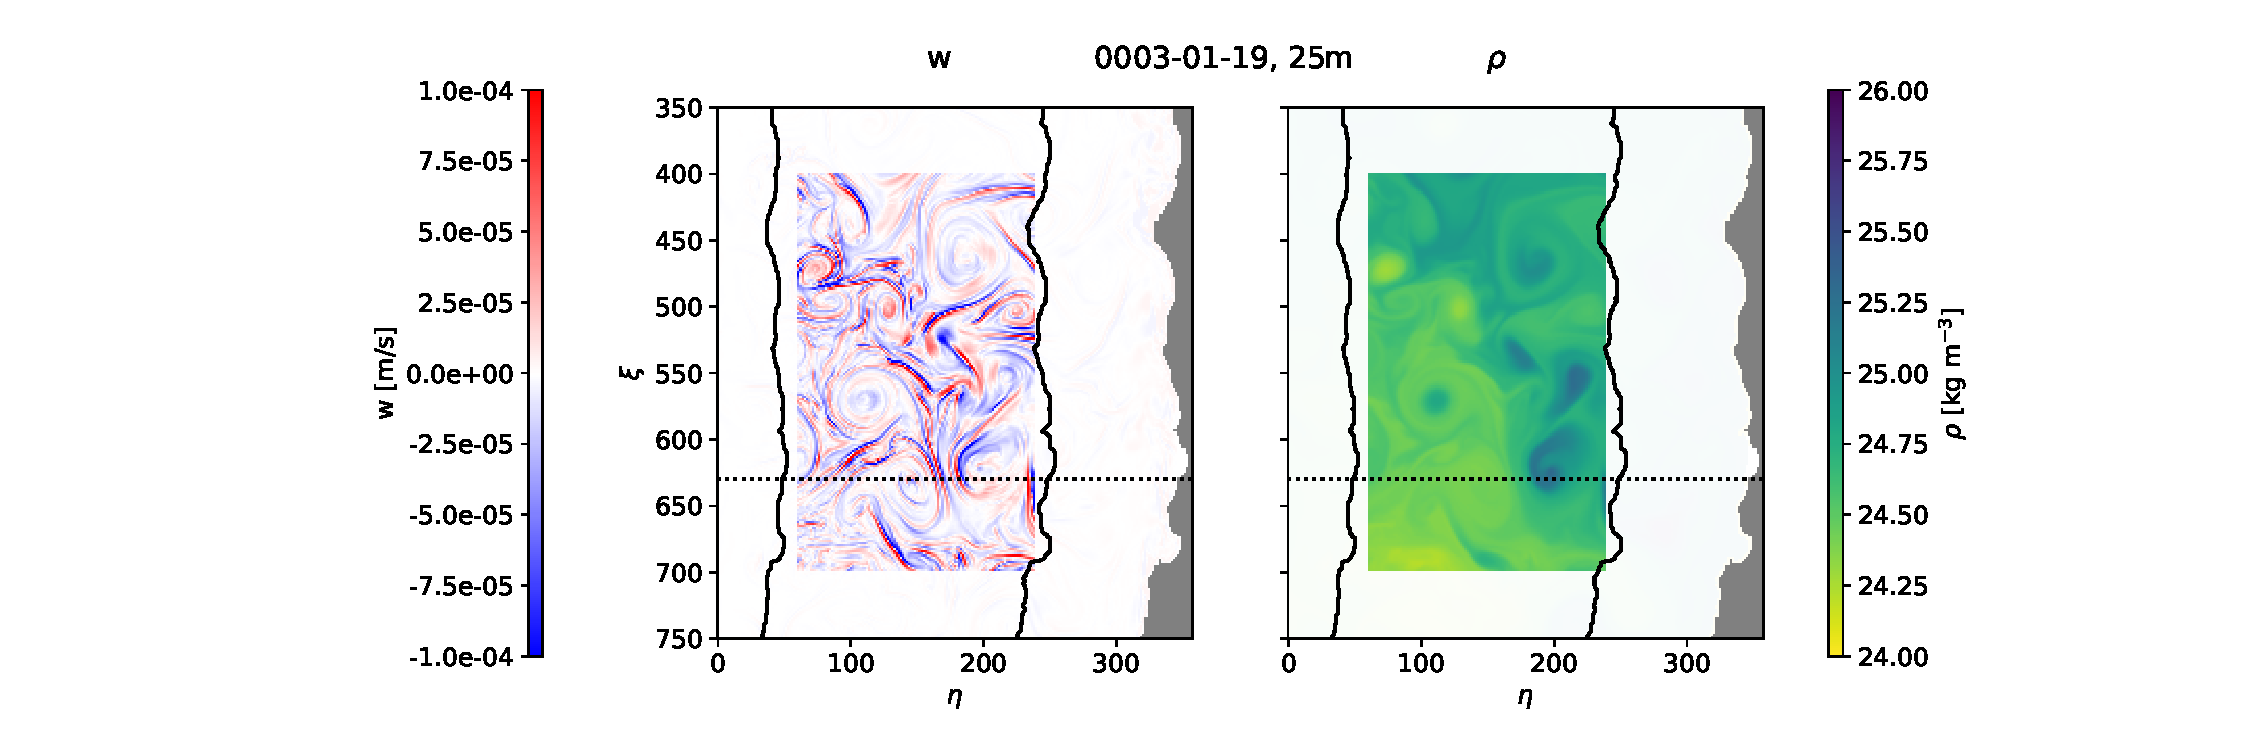
\includegraphics[width=17cm, trim=5.2cm 0 0 0]{../figures/result_subm_snapshot-p15}
    \caption[Snapshot of submesoscale fronts in HR]{\textbf{Snapshot of submesoscale fronts in HR}. The snapshot is from mid January at 25m depth and shows the vertical velocity (right) and density (left). The domain is in grid coordinates $\eta$ and $\xi$. The highlighted area is the area to which the detection algorithm is applied. Black solid lines represent $\SI{200}{\kilo\metre}$ and $\SI{800}{\kilo\metre}$ distance from coast. The dotted line is the location of the vertical section shown in \autoref{fig:subm-sample-vertical}.}\label{fig:subm-sample-hr}
\end{figure}
\begin{figure}
    \centering
    \hspace*{-0.17cm}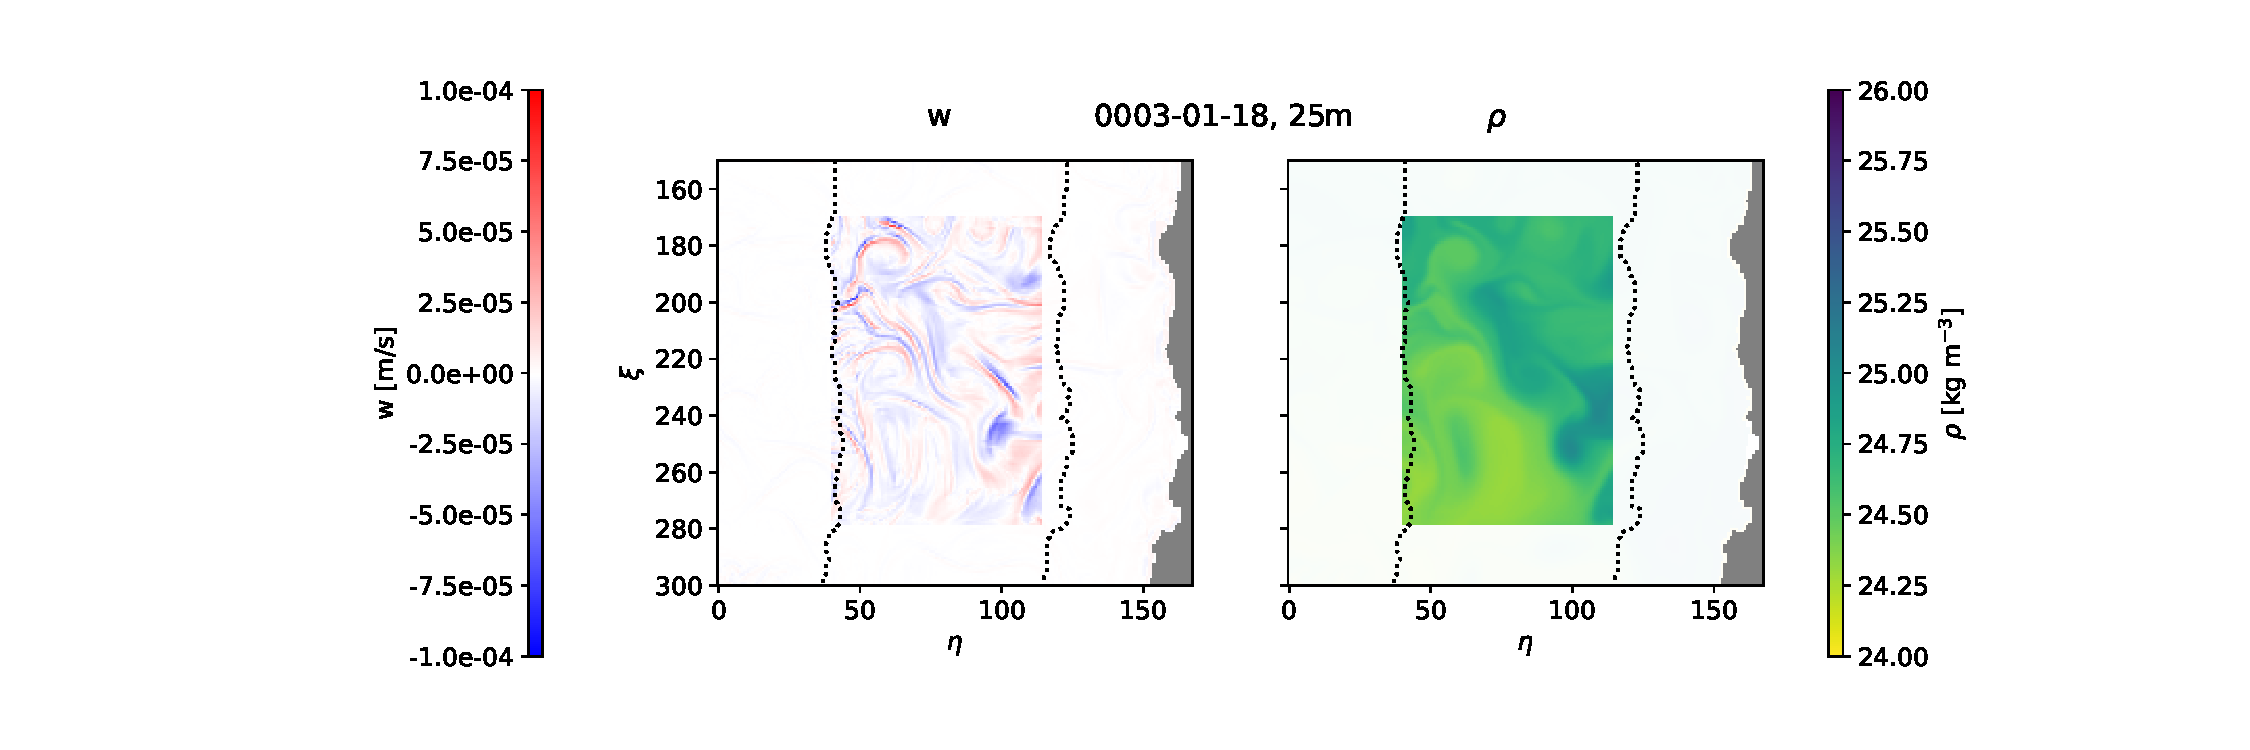
\includegraphics[width=17cm, trim=5.2cm 0 0 0]{../figures/result_subm_snapshot-p30}
    \caption[Snapshot of submesoscale fronts in MR]{\textbf{Snapshot of submesoscale fronts in MR}. See \autoref{fig:subm-sample-hr} for explanations.}\label{fig:subm-sample-lr}
\end{figure}
\\
Submesoscale fronts are located at steep, outcropping isopycnals. This can be seen in \autoref{fig:subm-sample-vertical} which shows the vertical section of the vertical velocity in the offshore region. The vertical velocity is always negative (downward) at the dense side of the density front and positive at the less dense side which is characteristic for frontogenesis \autocite{thomas-2008-subm}. Further, it shows exemplarily that most of the fronts can be found between mesoscale eddies. This emphasizes the importance of eddy-induced strain for frontogenesis \autocite{thomas-2008-subm}.\\
\begin{figure}
    \centering
    \hspace*{0.7cm}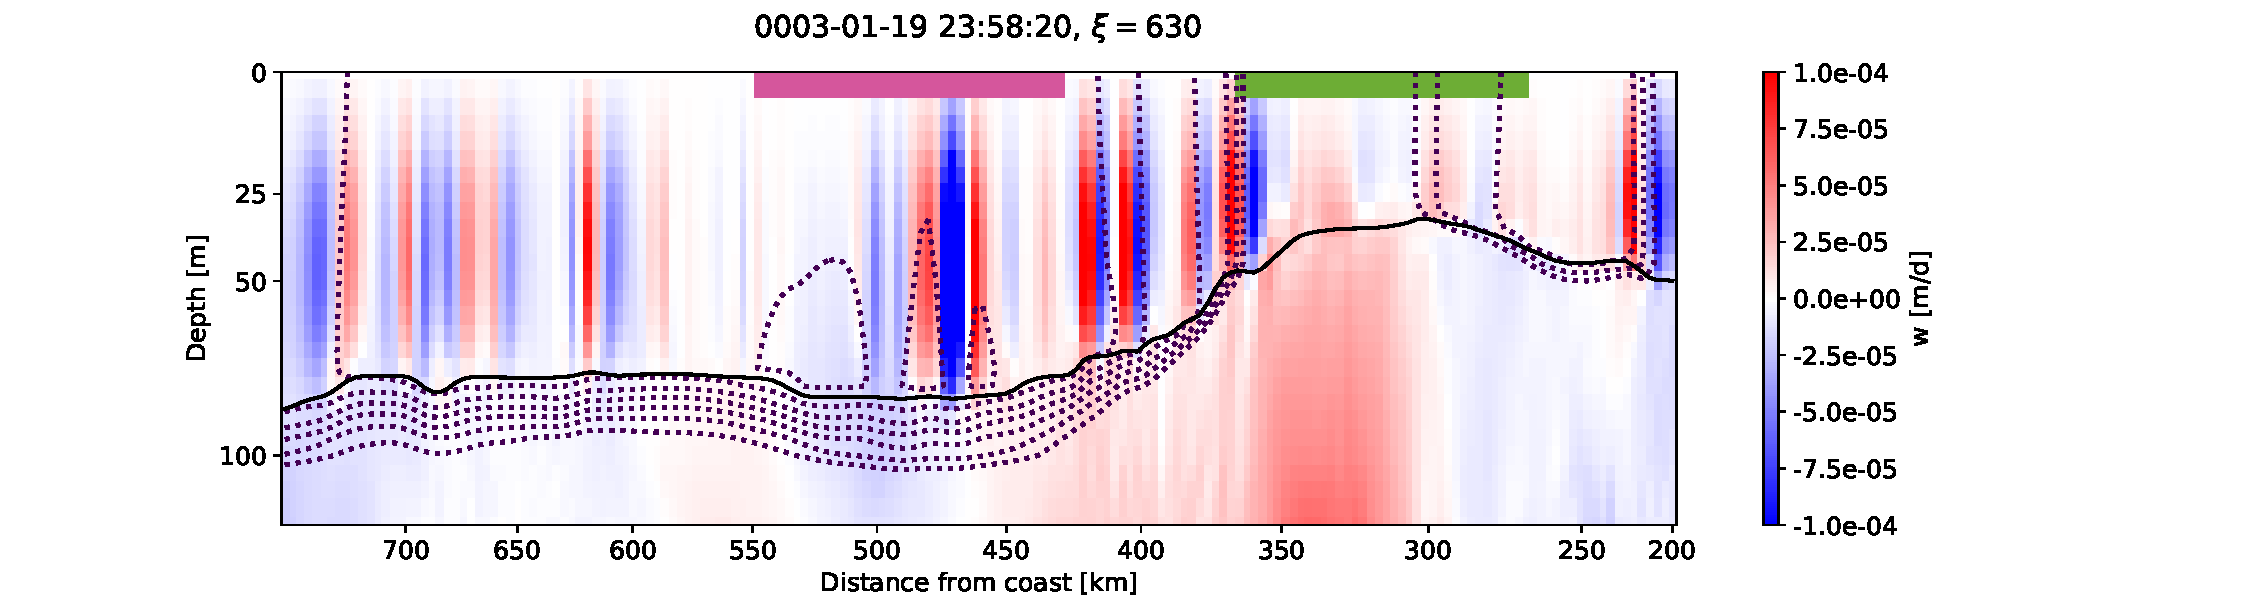
\includegraphics[width=17cm, trim=2.3cm 0 0 0]{../figures/result_snapshot-vert-p15}
    \caption[Vertical section of submesoscale fronts]{\textbf{Vertical section of submesoscale fronts}. The solid black line represents the \ac{mld}, dotted black lines show isopycnals. The green bars denote cyclones, pink bars anticyclones (positions from \autoref{sec:mesoscale-comparison}).}\label{fig:subm-sample-vertical}
\end{figure}
\\
\\
Submesoscale fronts range from the surface to the base of the mixed layer and only few reach below it (see \autoref{fig:subm-sample-vertical}). Therefore, their presence is strongly modulated by the seasonality of the \ac{mld} which is driven by atmospheric forcing. The \ac{mld} is deepest in winter and shallowest in summer \autocite{callies-2015-seasonality-subm}. Also submesoscale fronts in \ac{mr} and \ac{hr} are strongest during winter, whereas only little activity is present during summer.\\
\\
Submesoscale fronts disappear after several days either by getting weaker or due to \ac{mli}. The former happens when the front is not stabilized (e.g. by mesoscale strain or down front winds), because the vertical velocities act to dampen the density front \autocite{thomas-2008-subm}. On the other hand, \ac{mli} arise when the front is stabilized or further intensified \autocite{boccaletti-2007}. Both mechanisms occur in \ac{hr} which is shown in \autoref{fig:subm-sample-mli}. The front is stable in the first snapshot whereas $\SI{10}{\day}$ later the front disperse to small \ac{mle} (visible in vorticity field).
\begin{figure}[h]
    \centering
    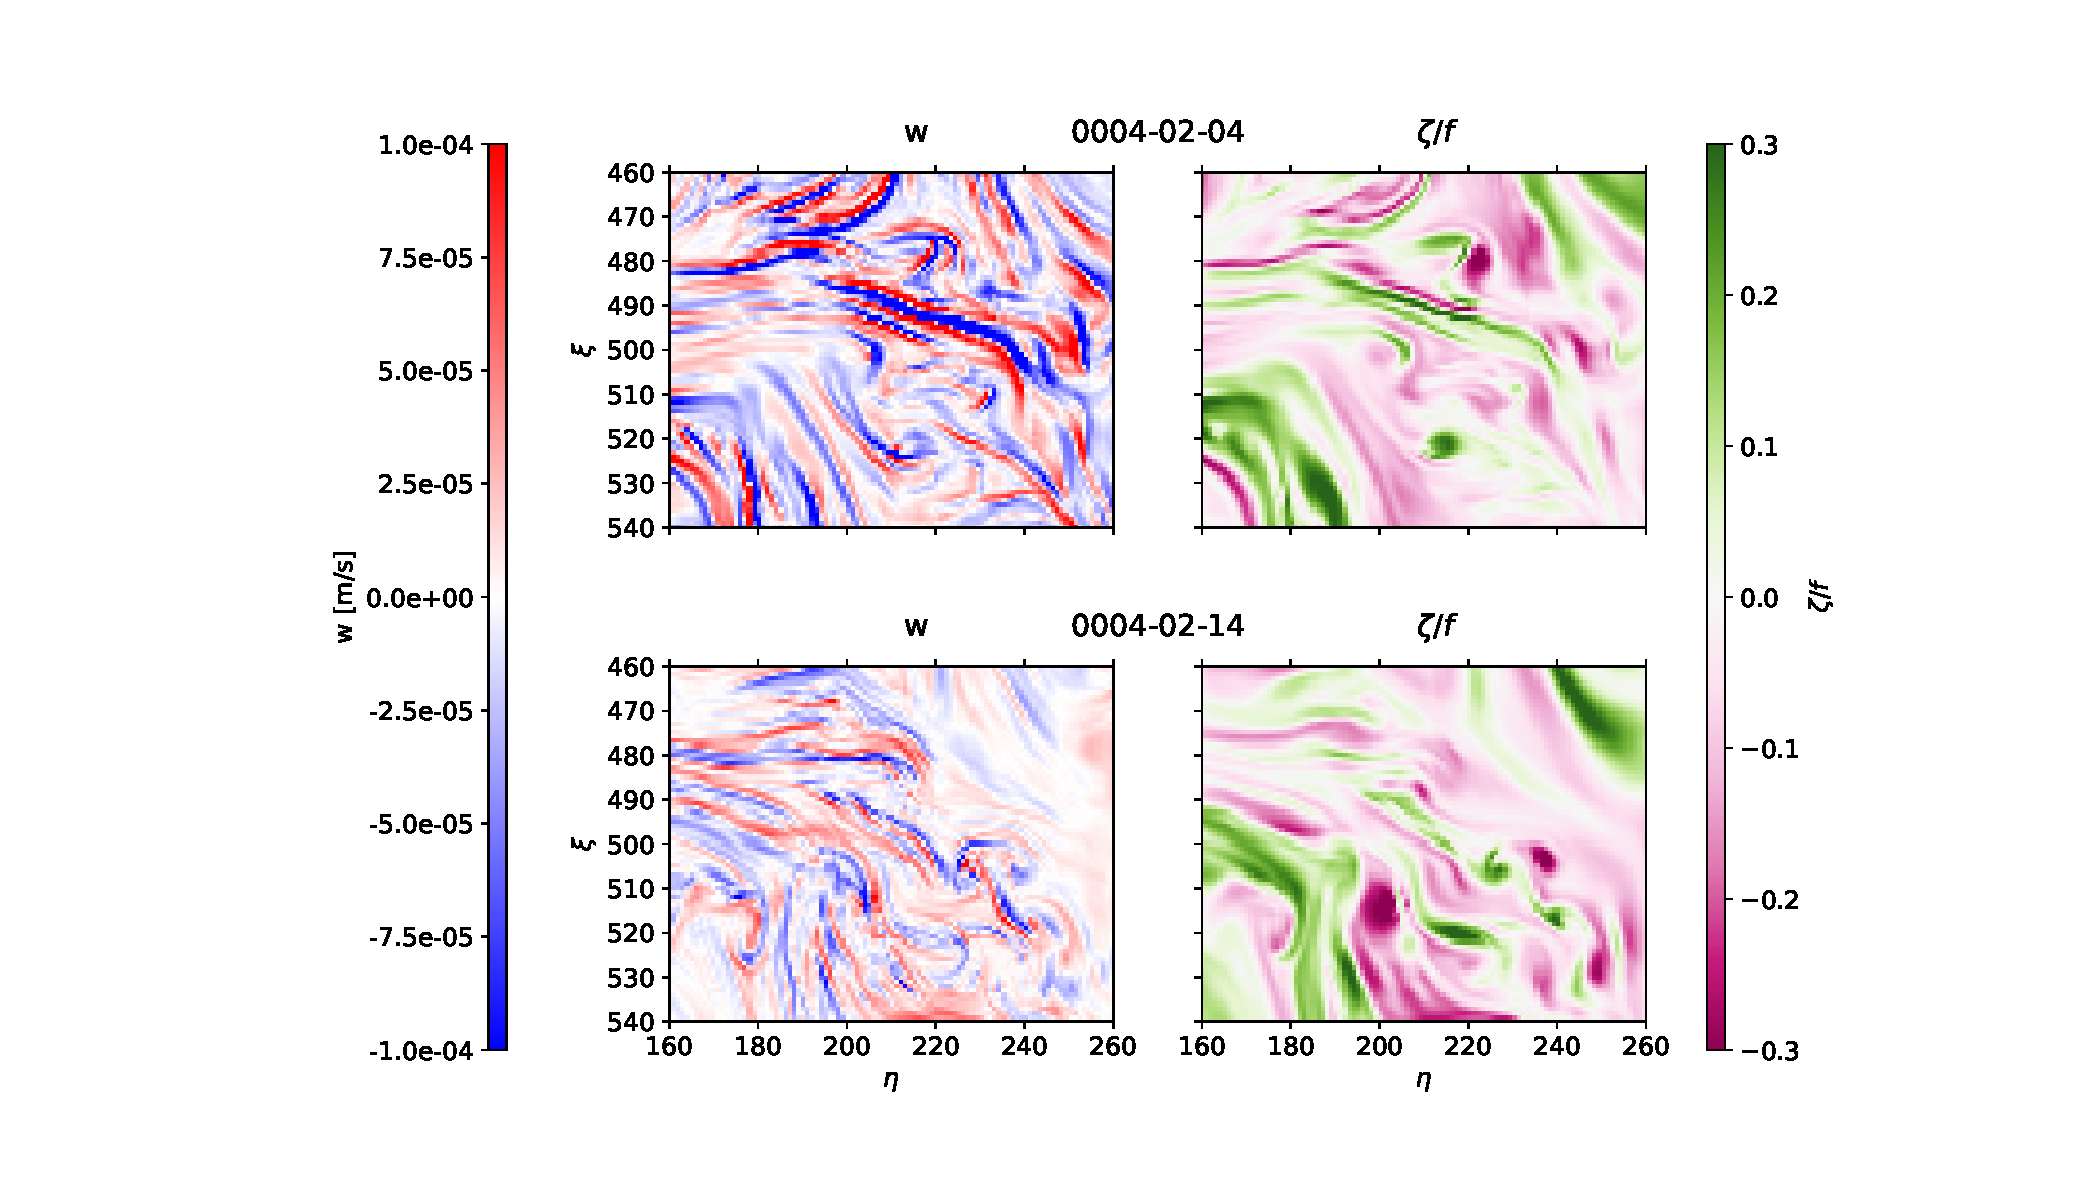
\includegraphics[width=16cm, trim=4cm 0 0 0]{../figures/result_snapshot_instabilities}
    \caption[Instabilities in submesoscale fronts]{\textbf{Instabilities in submesoscale fronts}. Vertical velocity (left) and vorticity (normalized by $f$, right) at $\SI{25}{\metre}$ depth. The top row shows a snapshot from early February, the bottom row is ten days later.}\label{fig:subm-sample-mli}
\end{figure}

\subsection{Submesoscale Front Detection}\label{sec:subm-detection}

In order to quantify the findings of \autoref{sec:subm-appearance}, a detection algorithm was developed to automatically detect submesoscale fronts in every snapshot. The algorithm makes use of three characteristics of submesoscale fronts: large vertical velocities, elongated spatial structure and consistency in depth. The method is described in detail in \autoref{sec:data-methods-submdet}.\\
\\
The detection algorithm reveals, that submesoscale fronts cover larger parts of the offshore region in \ac{hr} than in \ac{mr}, especially at the base of the mixed layer. During winter, submesoscale fronts cover $\SI[separate-uncertainty]{14.0(1)}{\percent}$ of the upper $30\text{m}$ of the considered domain in \ac{mr} and $\SI[separate-uncertainty]{16.2(1)}{\percent}$ in \ac{hr}. The difference between \ac{mr} and \ac{hr} increases at greater depths. When considering the $\SI{10}{\metre}$ around the \ac{mld} (calculated for each day as domain average), only $\SI[separate-uncertainty]{5.3(1)}{\percent}$ of the domain in \ac{mr} is covered by submesoscale fronts whereas $\SI[separate-uncertainty]{10.1(1)}{\percent}$ is covered in \ac{hr}. The coverage is also visualized in \autoref{fig:subm-coverage}. The data shown in the plot also confirm the qualitatively observed modulation by the \ac{mld} as well as the seasonal cycle of submesoscale fronts. From these results, it can be concluded that submesoscale fronts are much better resolved in \ac{hr}. Therefore, the following part refers only to \ac{hr}.\\
\begin{figure}[h]
    \centering
    \hspace*{-0.17cm}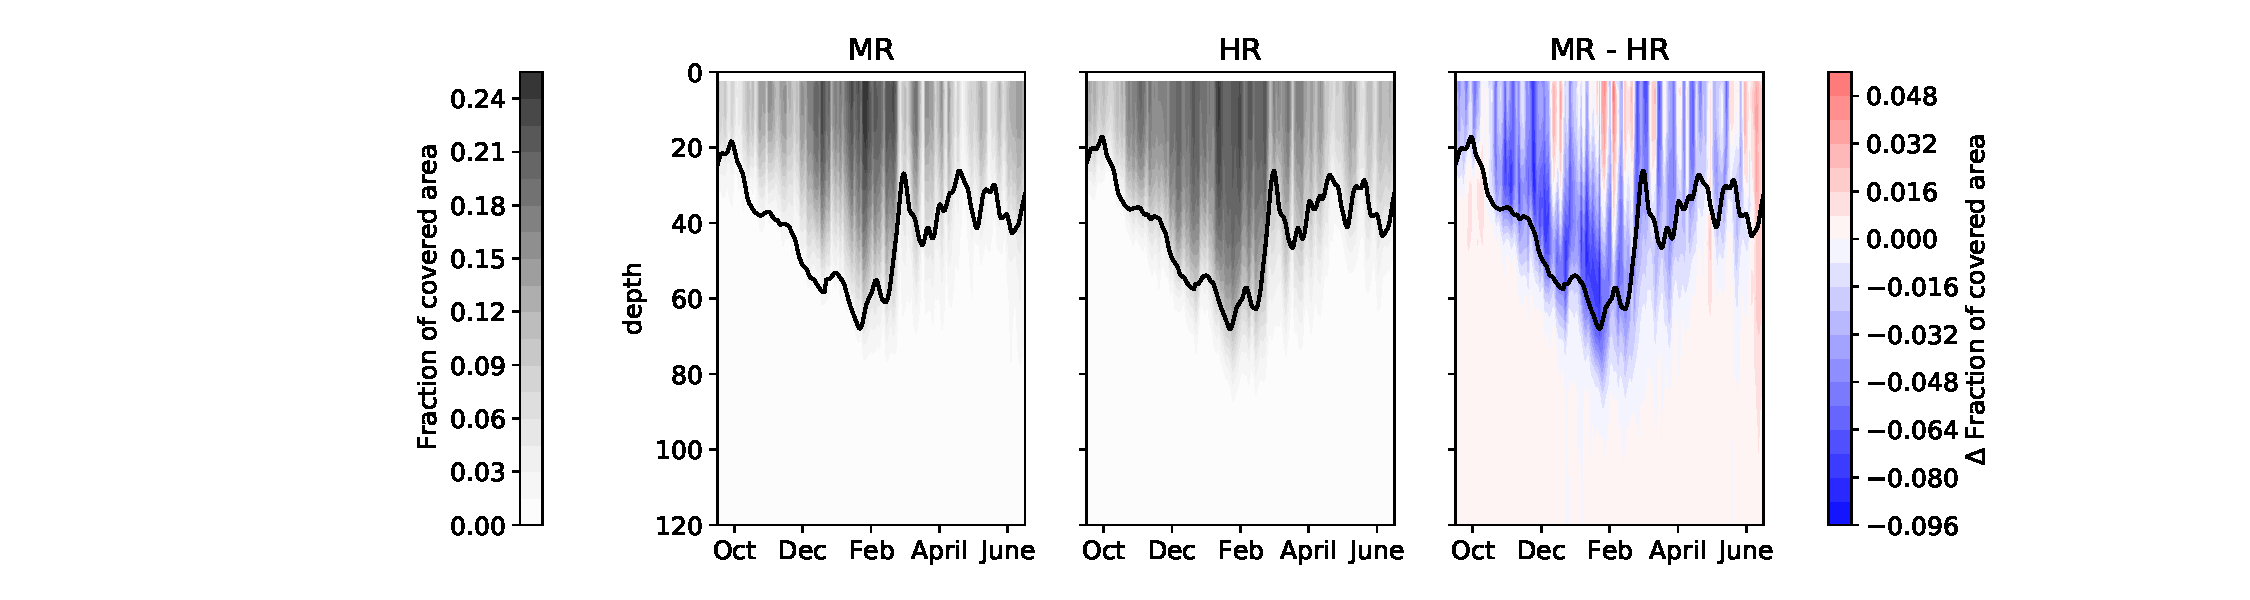
\includegraphics[width=17cm, trim=6cm 0 0 0]{../figures/result_subm_coverage.pdf}
    \caption[Area covered by submesoscale fronts]{\textbf{Area covered by submesoscale fronts} relative to total area. \ac{mr} is shown left, \ac{hr} in the center. The difference \ac{mr} - \ac{hr} is shown right. The solid line denotes the average \ac{mld}}\label{fig:subm-coverage}
\end{figure}
\\
The detection algorithm reveals a slight asymmetry between upwelling and downwelling fronts. The area covered by upwelling fronts is on average $\SI[separate-uncertainty]{3.1(6)}{\percent}$ larger than the area covered by downwelling fronts. Further, the average downwelling velocity ($\SI[separate-uncertainty]{-2.94(1)}{\metre\per\day}$) is $\SI{8.9(3)}{\percent}$ larger than the upwelling velocity ($\SI[separate-uncertainty]{2.65(1)}{\metre\per\day}$). This asymmetry is indeed expected for submesoscale frontogenesis \autocite{mahadevan-2006-subm-fronts-asym}. The occurrence of the asymmetry in the detection results indicates that the algorithm is capable of detecting the fronts quite precisely.\\
\\
Submesoscale fronts impact mesoscale anticyclones stronger than cyclones. Overall, fronts appear mainly outside of mesoscale eddies: during winter, $\SI[separate-uncertainty]{75.1(14)}{\percent}$ of the area associated with submesoscale fronts is located outside of mesoscale eddies, albeit the eddies cover $\SI[separate-uncertainty]{31.3(34)}{\percent}$ of the domain. The remaining area is distributed on mesoscale eddies with $\SI[separate-uncertainty]{10.3(4)}{\percent}$ occurring in cyclones and $\SI[separate-uncertainty]{14.5(4)}{\percent}$ in anticyclones. This difference is particularly interesting, because cyclones cover a majority of $\SI[separate-uncertainty]{63.1(73)}{\percent}$ of the area associated with mesoscale eddies during this time. As a result, only $\SI[separate-uncertainty]{8.3(5)}{\percent}$ of the area associated with cyclones intersect with submesoscale fronts whereas $\SI[separate-uncertainty]{20.0(9)}{\percent}$ of the anticyclonic area do. Furthermore, submesoscale fronts occur in anticyclones not only at the eddy edge (as they do in cyclones) but also inside the eddy core. This can be seen in composites of the absolute vertical velocity in \autoref{fig:subm-wabs}. The composites are only based on mesoscale eddy detection and thus confirm the finding independently from the detection algorithm for submesoscale fronts.\\
\begin{figure}[h]
    \centering
    \hspace*{0.3cm}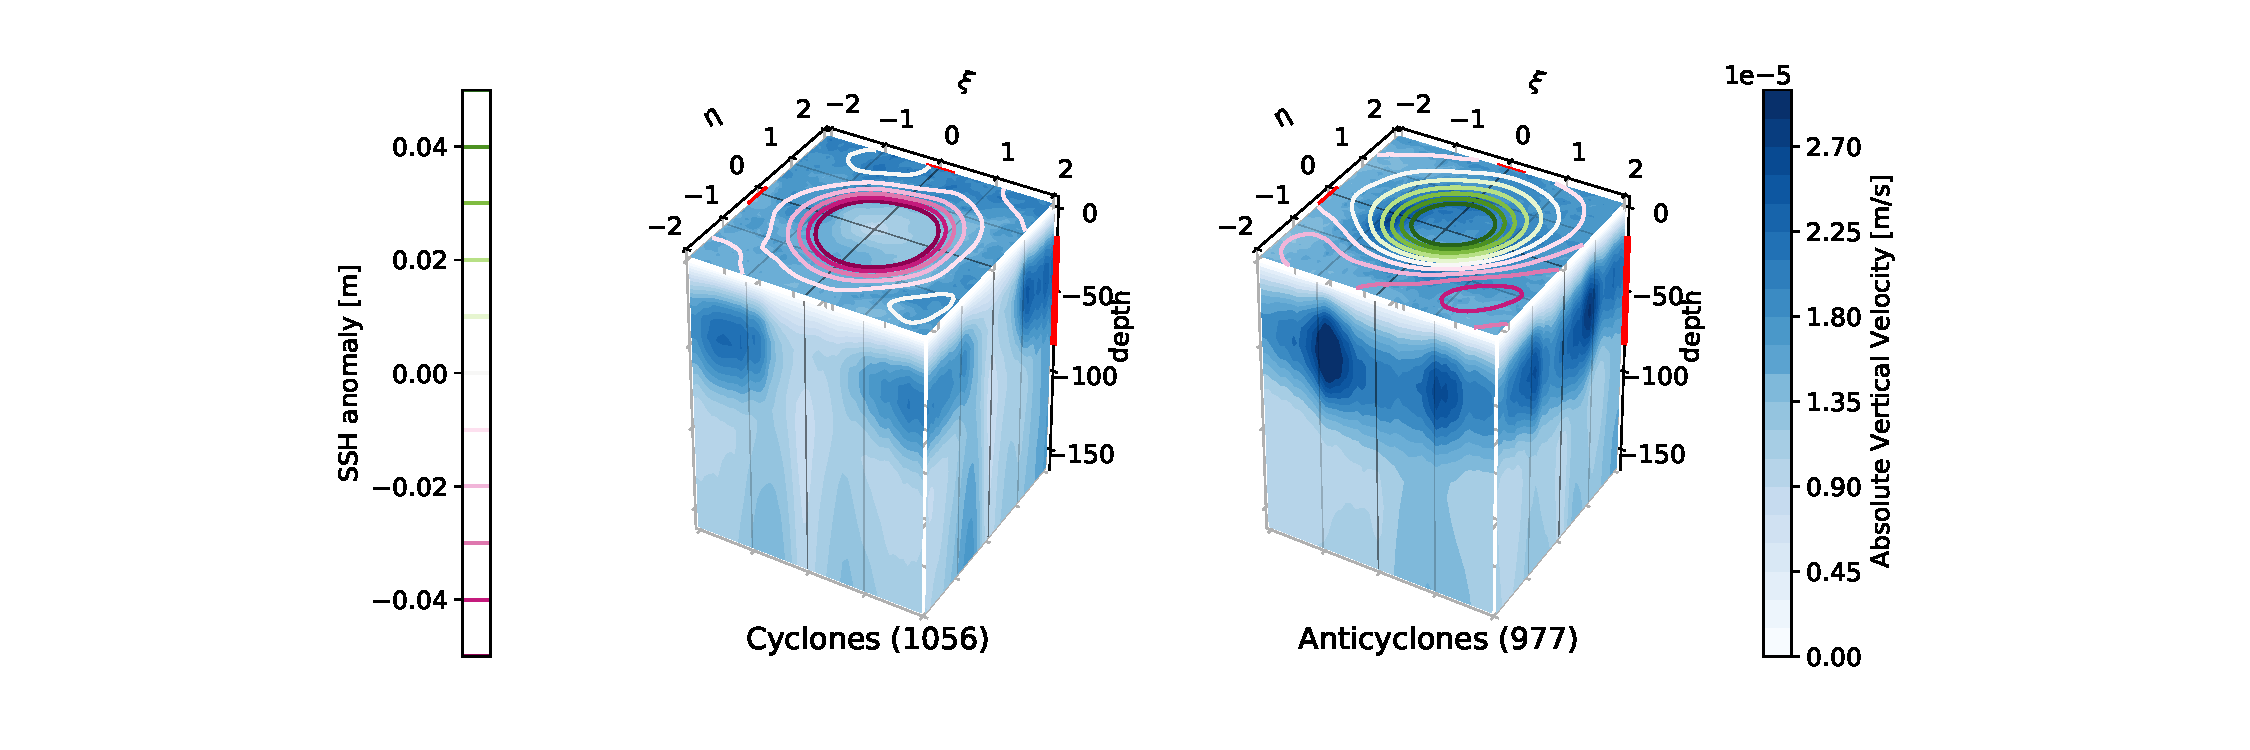
\includegraphics[width=17cm, trim=5cm 0 0 0]{../figures/result_composites_w-abs-p15}
    \caption[Vertical velocity anomaly in HR]{\textbf{Vertical velocity anomaly in HR}. Composite for cyclones is shown left and for anticyclones right. Only offshore eddies from January to March were considered. Contours on top represent SSH anomalies. The surfaces are averages of the perpendicular axes, the range for the averages are shown in red on the axes. The number of aggregated eddies is denoted in brackets.}\label{fig:subm-wabs}
\end{figure}
\\
\\
In contrast, the interaction of submesoscale fronts with mesoscale eddies, especially anticyclones, is much weaker in \ac{mr}: only $\SI[separate-uncertainty]{7.0(6)}{\percent}$ of cyclones and $\SI[separate-uncertainty]{11.7(5)}{\percent}$ of anticyclones are covered by submesoscale fronts. Accordingly, the vertical velocities inside the eddies are also less affected (see \autoref{fig:subm-wabs-meso} in comparison to \autoref{fig:subm-wabs}).\\
\begin{figure}
    \centering
    \hspace*{0.3cm}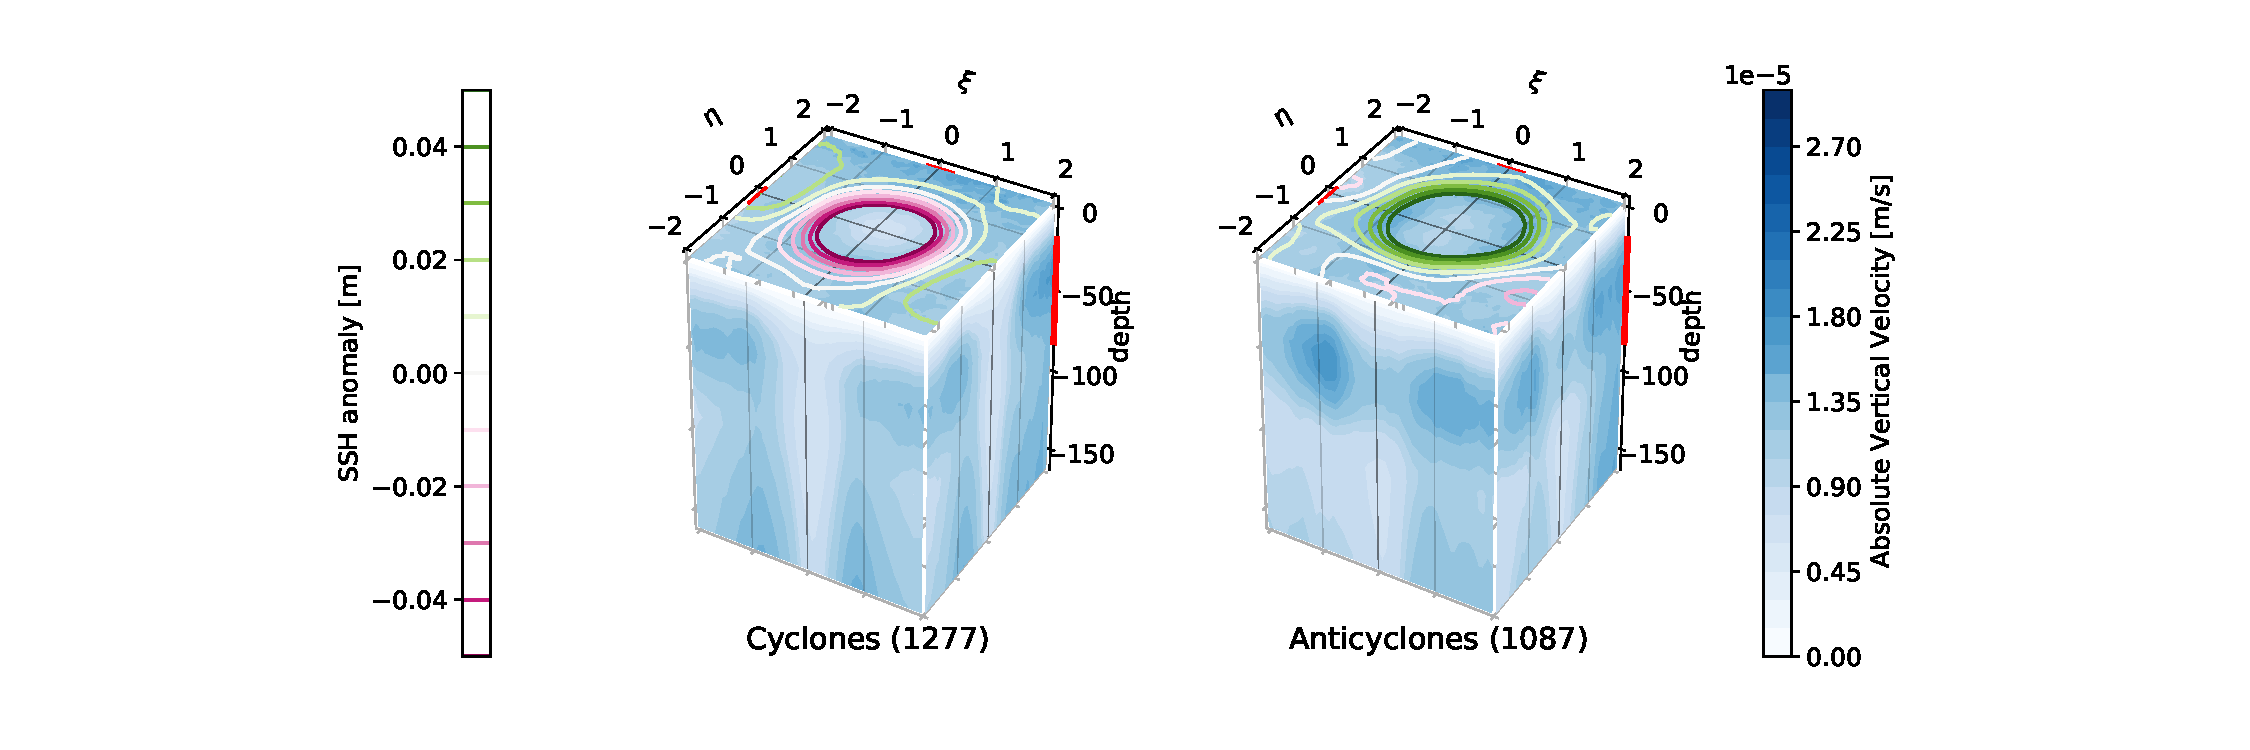
\includegraphics[width=17cm, trim=5cm 0 0 0]{../figures/result_composites_w-abs-p30}
    \caption[Vertical velocity anomaly in MR]{\textbf{Vertical velocity anomaly in MR}. See \autoref{fig:subm-wabs} for explanations.}\label{fig:subm-wabs-meso}
\end{figure}
\\
In summary, the process of submesoscale frontogenesis is much better resolved in \ac{hr} than in \ac{mr}. The appearance in \ac{hr} matches well to theoretical expectations (see \autoref{sec:introduction}) or observations from previous studies (e.g. \textcite{capet-2008-fronts2}). Even \ac{mle} can be observed in \ac{hr}, albeit this is very close to the resolution limit. Furthermore, results of the detection algorithm confirm that fronts are modulated by the \ac{mld} and that they are most active during winter. In addition, a strong intersection of submesoscale fronts and mesoscale eddies can be detected in \ac{hr}. At this, especially anticyclones are affected. This asymmetry is discussed in detail in \autoref{sec:discussion}.